%==============================================================================
% Poster - Arno Verhulst
%==============================================================================
\documentclass[a0,portrait]{hogent-poster}
\usepackage{xcolor}
\usepackage{graphicx}
\usepackage{caption}

% Laad tcolorbox stabiel in met extra bibliotheken voor schaduw en effecten
\usepackage[most]{tcolorbox}

% Professioneel kleurenpalet
\definecolor{posterbg}{HTML}{E9F0F8}     % Zachte achtergrondkleur voor de poster
\definecolor{cardblue}{HTML}{1A5276}     % Diepblauw voor de primaire kaarthoofden
\definecolor{cardbg}{HTML}{FFFFFF}       % Smetteloos wit voor de inhoud van de kaarten
\definecolor{accentorange}{HTML}{D35400} % Accentkleur voor de belangrijkste resultaten
\definecolor{darkslate}{HTML}{2C3E50}    % Donkergrijs voor de samenvatting

% Badges
\newcommand{\badge}[1]{\tcbox[on line, sharp corners=all, arc=1mm, colback=posterbg, colframe=cardblue, boxrule=0.3mm, top=1mm, bottom=1mm, left=2mm, right=2mm]{\small\bfseries\color{cardblue}#1}}
\newcommand{\badgeorange}[1]{\tcbox[on line, sharp corners=all, arc=1mm, colback=accentorange!10, colframe=accentorange, boxrule=0.3mm, top=1mm, bottom=1mm, left=2mm, right=2mm]{\small\bfseries\color{accentorange}#1}}

% Onderzoekskaarten via tcolorbox
\newtcolorbox{onderzoekskaart}[2][]{%
    enhanced,
    colback=cardbg,
    colframe=#2,
    coltitle=white,
    fonttitle=\bfseries\large,
    title={#1},
    boxrule=0mm,          % Geen storende buitenranden
    titlerule=0mm,
    toptitle=10mm,        % Ruime ademruimte boven de titel
    bottomtitle=10mm,     % Ruime ademruimte onder de titel
    top=12mm,             % Content padding aan de binnenkant
    bottom=12mm,
    left=12mm,
    right=12mm,
    arc=5mm,              % Prachtige, subtiele afronding
    boxsep=0mm,
    before skip=0mm,
    after skip=1.5cm,     % Vaste, gelijke afstand onder elke kaart
    shadow={5mm}{-5mm}{0mm}{black!8} % Subtiele schaduw voor diepte en modern design
}

% Info over de opleiding
\course{Bachelorproef}
\studyprogramme{toegepaste informatica}
\academicyear{2025-2026}
\institution{Hogeschool Gent, Valentin Vaerwyckweg 1, 9000 Gent}

% Info over de bachelorproef
\title{Optimalisatie van de Recovery Time Objective (RTO)}
\subtitle{in Active-Passive High Availability Clusters met Pacemaker en Corosync op RHEL-Nodes}
\author{Arno Verhulst}
\email{arno.verhulst@student.hogent.be}
\supervisor{Dhr. P. Beke}
\cosupervisor{Dhr. D. Allaert}

\specialisation{IT Infrastructure Engineer}
\keywords{High Availability, Cloud Gap, Pacemaker, Corosync, RTO-Optimalisatie, Fencing}
\projectrepo{https://github.com/vharno1612/bachelorproef-2526-vharno1612.git}

\begin{document}
   
    \pagecolor{posterbg}
    
    \maketitle
    
    % Abstract / Samenvatting
    \begin{center}
        \begin{minipage}{0.96\linewidth}
            \begin{onderzoekskaart}[SAMENVATTING]{darkslate}
                \large In de huidige digitale samenleving veroorzaakt ongeplande downtime van vitale webapplicaties zware financiële en reputatieschade. Hoewel open-source technologieën zoals Pacemaker en Corosync een robuuste basis bieden, voldoet de standaardconfiguratie niet aan de strenge RTO-eisen in de cloud. Door een gecoördineerde parameter-optimalisatie op het niveau van de clusterstack, Linux TCP-stack en Azure-netwerklaag werd de hersteltijd bij een node-uitval drastisch gereduceerd. Dit resulteerde in een transitie van een falende failover naar een gemiddelde RTO van slechts \textbf{1,33 tot 3,37 seconden}, wat een herstelverbetering van \textbf{$>$90\%} betekent.
            \end{onderzoekskaart}
        \end{minipage}
    \end{center}
    
    \vspace{0.5cm}
    
    % START VAN HET KOLOMMENRASTER
    \begin{center}
        \begin{minipage}{0.96\linewidth}
            
            \noindent
            % LINKERKOLOM
            \begin{minipage}[t]{0.489\linewidth}
                \vspace{0pt}
                
                % KAART 1: Onderzoeksvragen
                \begin{onderzoekskaart}[1. Onderzoeksvragen]{cardblue}
                    \begin{tcolorbox}[colback=posterbg, colframe=cardblue, boxrule=0.5mm, arc=3mm, top=5mm, bottom=5mm, left=5mm, right=5mm, shadow={3mm}{-3mm}{0mm}{black!5}]
                        \textbf{\color{cardblue}Hoofdonderzoeksvraag:}\\
                        \itshape Hoe kan een betaalbare Active-Passive High Availability webomgeving,
                        bestaande uit Pacemaker en Corosync op RHEL-compatibele nodes, geoptimaliseerd
                        worden om de RTO van de webapplicatie bij serveruitval te minimaliseren?
                    \end{tcolorbox}
                    
                    \vspace{0.2cm}
                    \noindent
                    {\small\color{cardblue}\itshape Onderstaande zinnen vatten de bijhorende deelvragen samen:}
                    
                    \vspace{0.2cm}
                    \noindent
                    % Sub-kolom 1: Probleemdomein
                    \begin{minipage}[t]{0.48\linewidth}
                        \vspace{0pt}
                        \textbf{\color{cardblue}Probleemdomein (Analyse):}
                        \begin{itemize}
                            \item Statusconsensus via Corosync, Pacemaker \& STONITH.
                            \item Identificatie van kritieke RTO-parameters \& constraints.
                            \item Risico's en beheer van virtuele IP-migratie.
                        \end{itemize}
                    \end{minipage}%
                    \hfill
                    % Sub-kolom 2: Oplossingsdomein
                    \begin{minipage}[t]{0.48\linewidth}
                        \vspace{0pt}
                        \textbf{\color{cardblue}Oplossingsdomein (Implementatie):}
                        \begin{itemize}
                            \item Split-brain preventie via Azure Power Fencing.
                            \item Kwantificering van RTO over 3 foutsituaties.
                            \item Iteratieve tuning vs. operationele stabiliteit.
                        \end{itemize}
                    \end{minipage}
                \end{onderzoekskaart}
                
                % KAART 2: Methodologie
                \begin{onderzoekskaart}[2. Methodologie \& Aanpak]{cardblue}
                    Het onderzoek werd uitgevoerd op de cloud-infrastructuur van \textbf{oXya Consulting BeNeLux} en is gestructureerd rond vier opeenvolgende fasen:
                    \vspace{0.6cm}
                    \begin{center}
                        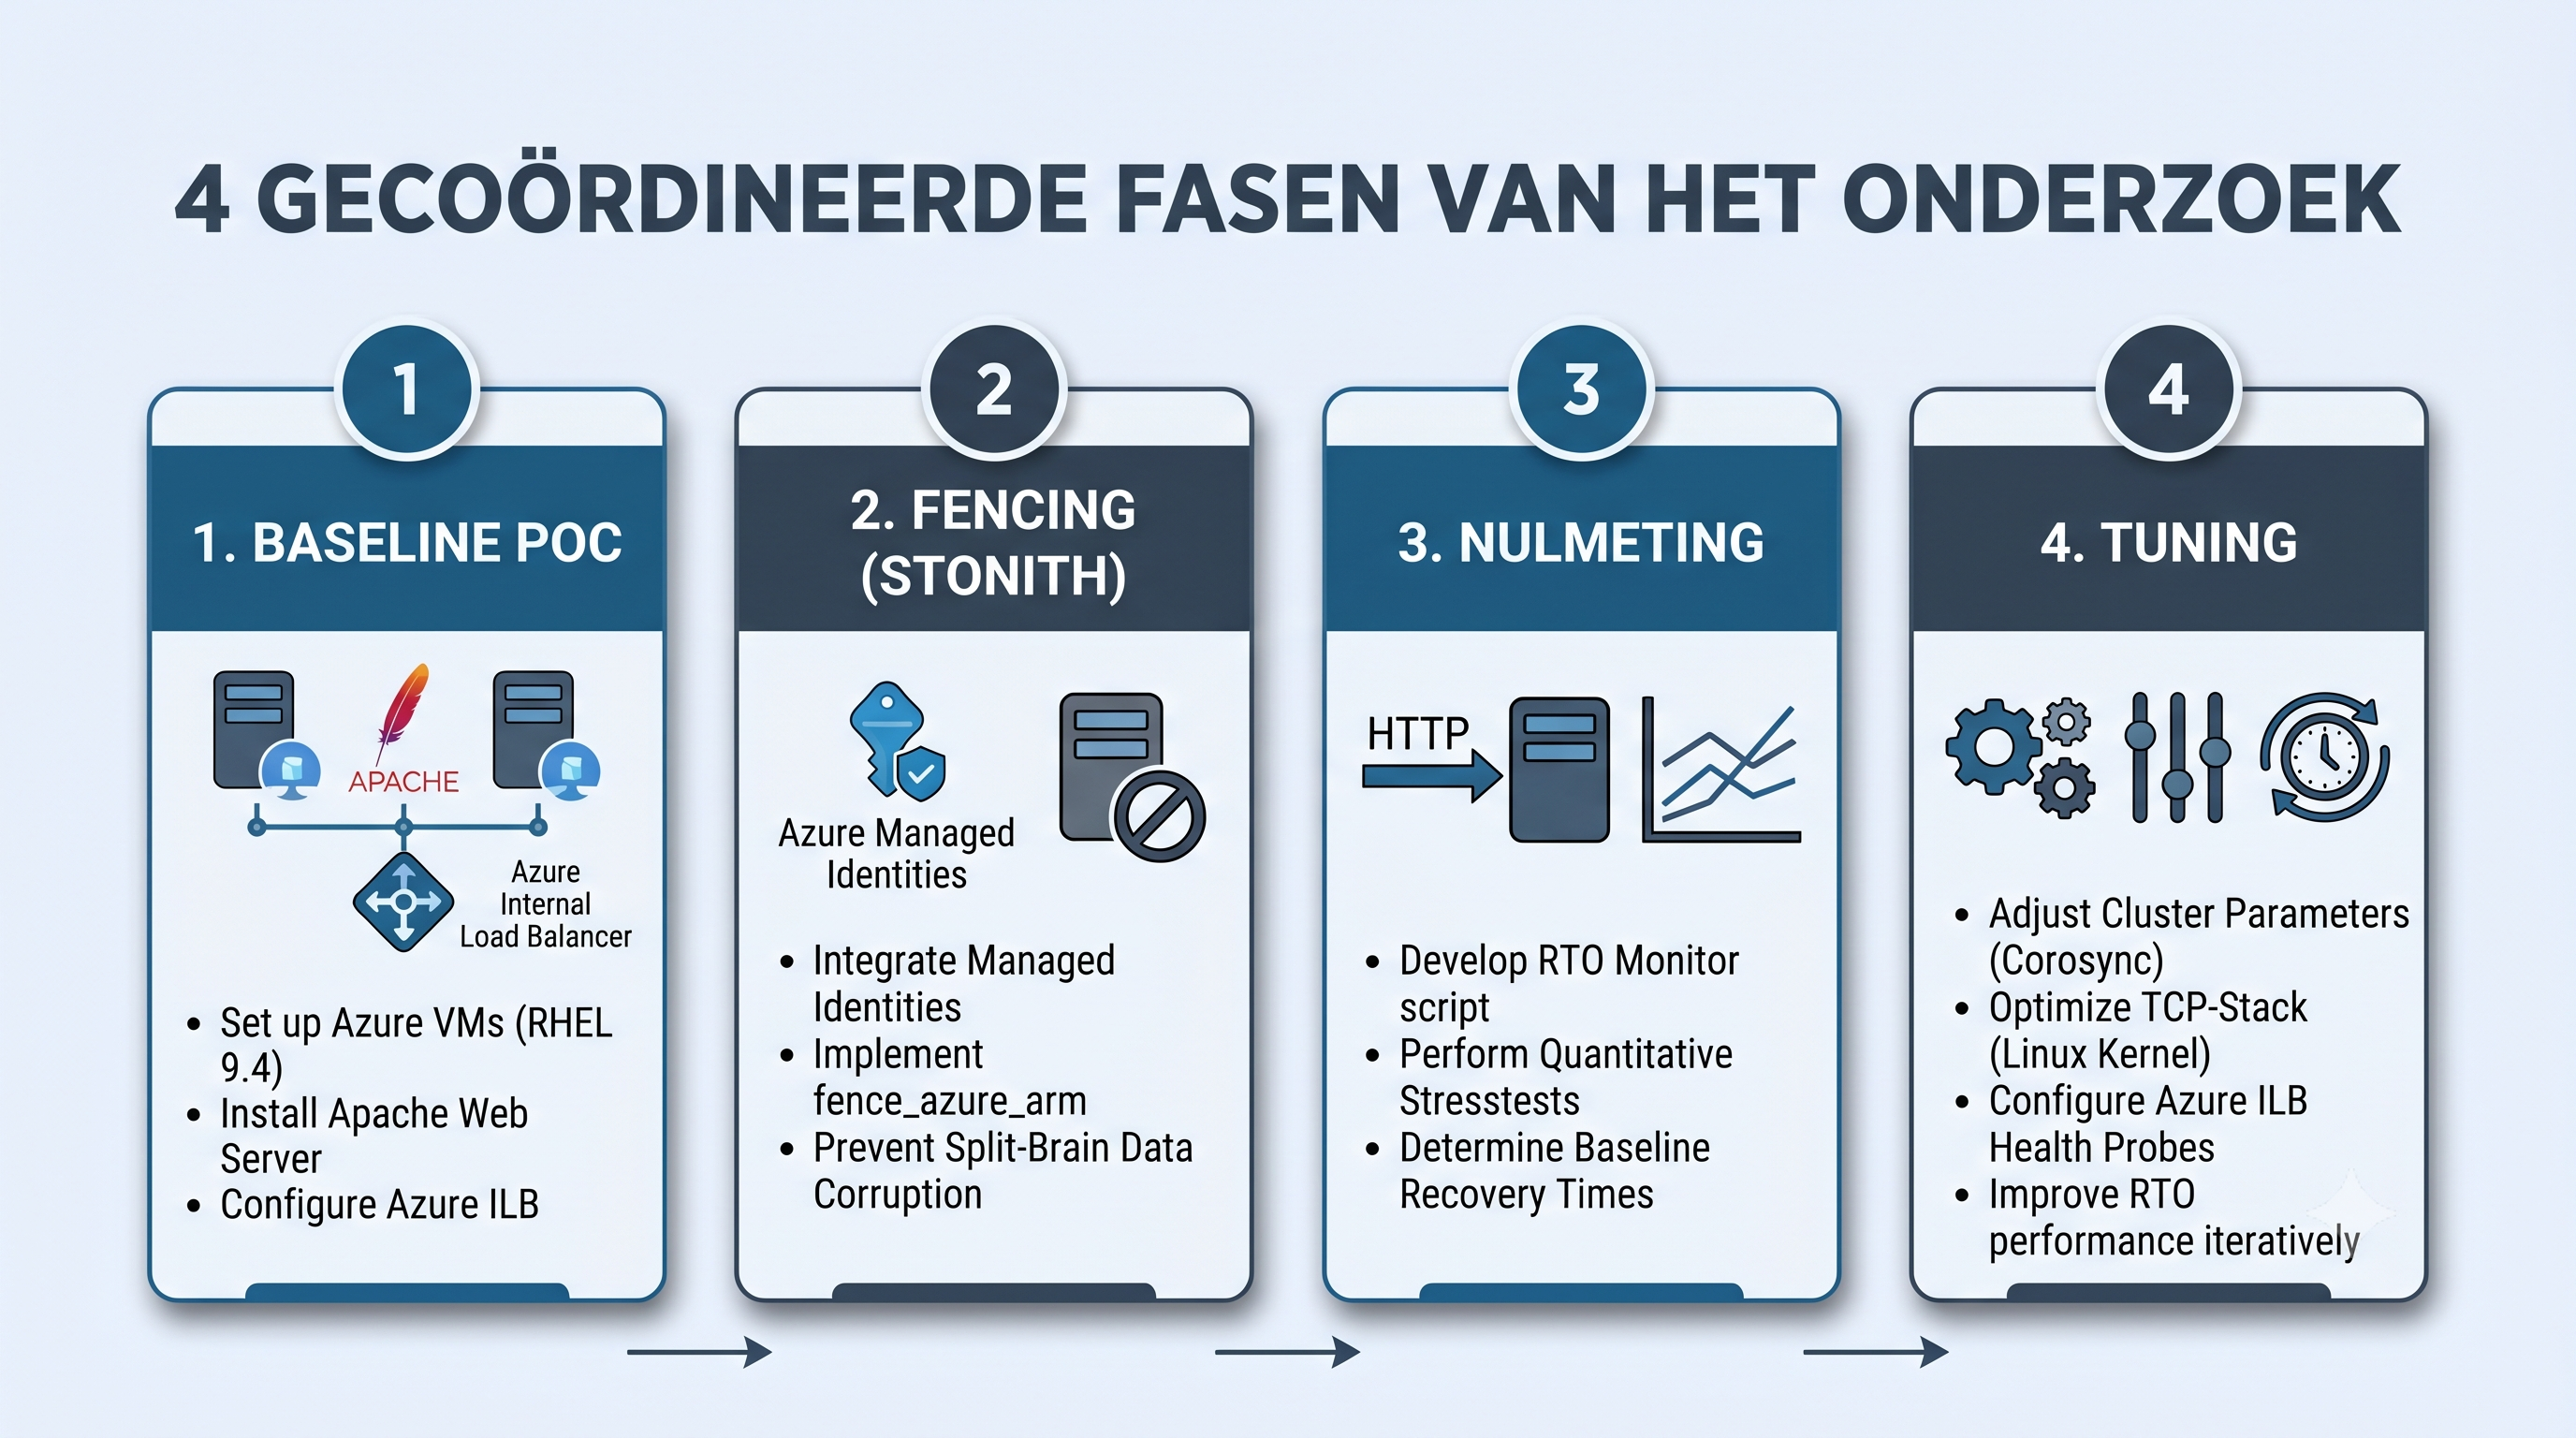
\includegraphics[width=1.0\linewidth]{graphics/methodologie} 
                        \vspace{0.4cm}
                        \captionof{figure}{Chronologische fasering van het onderzoek: van PoC-nulmeting tot iteratieve tuning. Eigen illustratie, gegenereerd met Gemini (Google), juni 2026.}
                    \end{center}
                \end{onderzoekskaart}
                
                % KAART 3
                \begin{onderzoekskaart}[3. Gecoördineerde Parameter-Tuning]{cardblue}
                    Om de hersteltijd te minimaliseren, zijn volgende parameters stapsgewijs geoptimaliseerd over drie gelaagde niveaus:
                    
                    \vspace{0.6cm}
                    \noindent
                    % Sub-kolom A
                    \begin{minipage}[t]{0.32\linewidth}
                        \vspace{0pt}
                        \textbf{\color{cardblue}A. Clusterstack}\\
                        \small\textit{(Corosync/Pacemaker)}
                        \begin{itemize}
                            \item \texttt{token}-timeout:\\ 3000ms $\rightarrow$ \badge{500ms}
                            \item Apache \texttt{monitor}:\\ 60s $\rightarrow$ \badge{2s}
                        \end{itemize}
                    \end{minipage}%
                    \hfill
                    % Sub-kolom B
                    \begin{minipage}[t]{0.32\linewidth}
                        \vspace{0pt}
                        \textbf{\color{cardblue}B. Linux Kernel}\\
                        \small\textit{(TCP-stack)}
                        \begin{itemize}
                            \item \texttt{tcp\_retries2}:\\ 15 $\rightarrow$ \badge{5}
                            \item \texttt{tcp\_syn\_retries}:\\ 6 $\rightarrow$ \badge{3}
                        \end{itemize}
                    \end{minipage}%
                    \hfill
                    % Sub-kolom C
                    \begin{minipage}[t]{0.32\linewidth}
                        \vspace{0pt}
                        \textbf{\color{cardblue}C. Cloud-Infra}\\
                        \small\textit{(Azure ILB)}
                        \begin{itemize}
                            \item Floating IP geactiveerd op OS.
                            \item Health Probe korter naar \badge{5s}
                        \end{itemize}
                    \end{minipage}
                \end{onderzoekskaart}
                
            \end{minipage}%
            \hfill 
            % RECHTERKOLOM 
            \begin{minipage}[t]{0.489\linewidth}
                \vspace{0pt} 
                
                % KAART 4: De Cloud Architectuur 
                \begin{onderzoekskaart}[4. Gelaagde Architectuur]{darkslate}
                    De geoptimaliseerde infrastructuur overbrugt de transitie van fysieke netwerkhardware naar software-defined networking binnen Microsoft Azure.
                    \begin{center}
                        
\includegraphics[width=1.0\linewidth]{netwerkschema} 
                        \vspace{0.4cm}
                        \captionof{figure}{Geoptimaliseerde Active-Passive infrastructuur binnen Azure. Overgenomen uit eigen bachelorproef; afbeelding gegenereerd met Gemini (Google), mei 2026.}
                    \end{center}
                    \nobreak
                \end{onderzoekskaart}
                
                % KAART 5: Resultaten
                \begin{onderzoekskaart}[5. Resultaten \& Teststatistieken]{accentorange}
                    De nulmeting toonde aan dat de standaardinstellingen faalden bij harde netwerkcrashes door een onbereikbare cloud-omgeving. Na optimalisatie zakten de RTO-tijden drastisch:
                    
                    \vspace{0.4cm}
                    \begin{center}
                        \small
                        \begin{tabular}{l|c|c|r}
                            \textbf{Uitvalscenario} & \textbf{RTO Baseline} & \textbf{RTO Opt.} & \textbf{Winst} \\
                            \hline
                            1. Service-level failure & 10,80s & \badgeorange{1,33s} & 87,7\% \\
                            2. Netwerkisolatie & $\infty$ (Faal) & \badgeorange{3,37s} & $>$99\% \\
                            3. Node-level crash & $\infty$ (Faal) & \badgeorange{2,03s} & $>$99\% \\
                        \end{tabular}
                        \captionof{table}{Kwantitatieve RTO-vergelijking voor en na tuning.}
                    \end{center}
                \end{onderzoekskaart}
                
                % KAART 6: Conclusie
                \begin{onderzoekskaart}[6. Conclusie \& Reflectie]{cardblue}
                    \begin{itemize}
                        \item[\textbf{\color{cardblue}$\bullet$}] \textbf{Optimalisatie:} Een integrale afstelling van de clusterstack, kernel en cloudinfrastructuur reduceert de RTO met meer dan 90\%.
                        \item[\textbf{\color{cardblue}$\bullet$}] \textbf{Integratie:} Het succesvol overbruggen van de 'Cloud Gap' via Floating IP is essentieel voor netwerkbeschikbaarheid in Azure.
                        \item[\textbf{\color{cardblue}$\bullet$}] \textbf{Risico:} De agressieve foutdetectie minimaliseert hersteltijden, maar introduceert een trade-off met netwerkstabiliteit.
                    \end{itemize}
                \end{onderzoekskaart}
                
            \end{minipage}
            
        \end{minipage}
    \end{center}
    
\end{document}